\documentclass[12pt,convert={false}]{standalone}
\usepackage[dvipsnames]{xcolor}
\usepackage{tikz}
\usetikzlibrary{shapes,arrows,positioning,calc,patterns,arrows.meta, bending, graphs, shadings,quotes,intersections}
\usetikzlibrary{external}
%\tikzexternalize[prefix=tikz/]
\usepackage{pgfplots}
\pgfplotsset{compat=1.16}
\usepgfplotslibrary{fillbetween}
\begin{document}
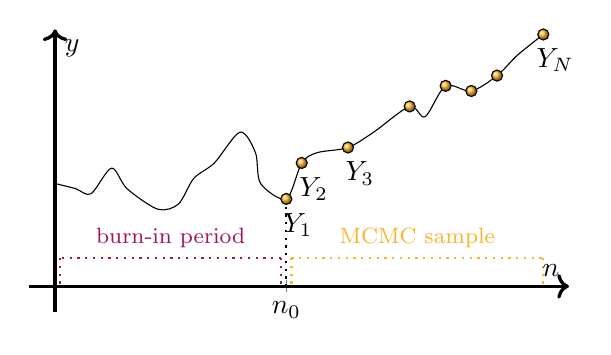
\begin{tikzpicture}
	\begin{axis}[
		axis lines=middle,
		unit vector ratio*=1 1 1,
		axis line style={->,very thick},
		xmin=-0.5,xmax=10,ymin=-0.5,ymax=5,
		xlabel=$n$,
		ylabel=$y$,
		xtick={0,4.5},
		ytick=\empty,
		xticklabels={0,$n_0$}
		]
		\addplot[smooth] coordinates {
			(0,2)
			(0.4,1.9)
			(0.7,1.8)
			(1.1,2.3)
			(1.4,1.9)
			(2,1.5)
			(2.4,1.6)
			(2.7,2.1)
			(3.1,2.4)
			(3.6,3)
			(3.9,2.6)
			(4,2)
			(4.5,1.7)
			(4.8,2.4)
			(5.1,2.6)
			(5.7,2.7)
			(6.2,3)
			(6.9,3.5)
			(7.2,3.3)
			(7.6,3.9)
			(8.1,3.8)
			(8.6,4.1)
			(9,4.5)
			(9.5,4.9)
		};
		\addplot [
		only marks,
		mark=ball,
		mark size=2pt,
		ball color=Dandelion,
		point meta=explicit symbolic,
		nodes near coords,
		every node near coord/.append style={xshift=0.15cm, yshift=-0.6cm},
		axis on top
		] coordinates {
			(4.5,1.7) [$Y_1$]
			(4.8,2.4) [$Y_2$]
			(5.7,2.7) [$Y_3$]
			(6.9,3.5)
			(7.6,3.9)
			(8.1,3.8)
			(8.6,4.1)
			(9.5,4.9) [$Y_N$]
		};
		\draw [Black,dotted,thick] (4.5,0) -- (4.5,1.7);
		\draw [dotted,thick,RedViolet] (4.4,0.55) -- (0.1,0.55) node[RedViolet,midway,above]{\footnotesize burn-in period};
		\draw [dotted,thick,RedViolet] (4.4,0.55) -- (4.4,0);
		\draw [dotted,thick,RedViolet] (0.1,0.55) -- (0.1,0);
		\draw [dotted,thick,Dandelion] (4.6,0.55) -- (9.5,0.55) node[Dandelion,midway,above]{\footnotesize MCMC sample};
		\draw [dotted,thick,Dandelion] (4.6,0.55) -- (4.6,0);
		\draw [dotted,thick,Dandelion] (9.5,0.55) -- (9.5,0);
	\end{axis}
\end{tikzpicture}
\end{document}
